%
% $RCSfile: knowledge_handling_system.tex,v $
%
% Copyright (c) 2005-2006. Christian Heller. All rights reserved.
%
% Permission is granted to copy, distribute and/or modify this document
% under the terms of the GNU Free Documentation License, Version 1.1 or
% any later version published by the Free Software Foundation; with no
% Invariant Sections, with no Front-Cover Texts and with no Back-Cover
% Texts. A copy of the license is included in the section entitled
% "GNU Free Documentation License".
%
% http://www.cybop.net
% - Cybernetics Oriented Programming -
%
% http://www.resmedicinae.org
% - Information in Medicine -
%
% Version: $Revision: 1.1 $ $Date: 2006-01-03 08:21:45 $ $Author: christian $
% Authors: Christian Heller <christian.heller@tuxtax.de>
%

\subsection{Knowledge-handling System}
\label{knowledge_handling_system_heading}

The pure existence of proper knowledge does not suffice to create an improved
kind of software system, within a slimmer software development process. The
system needs to know how to \emph{handle} knowledge, at runtime. The criticism
is twofold, since traditionally:

\begin{enumerate}
    \item Operating systems don't have sufficient knowledge handling capabilities
    \item Applications contain too much low-level system control functionality
\end{enumerate}

This is changed when using CYBOI. As active interpreter encapsulating
system-level functionality, it handles knowledge provided in form of passive
CYBOL templates. In CYBOP systems, all compound knowledge models have the same
type structure (schema). Since they do not differ, they can be manipulated in
the same manner.

\begin{figure}[ht]
    \begin{center}
        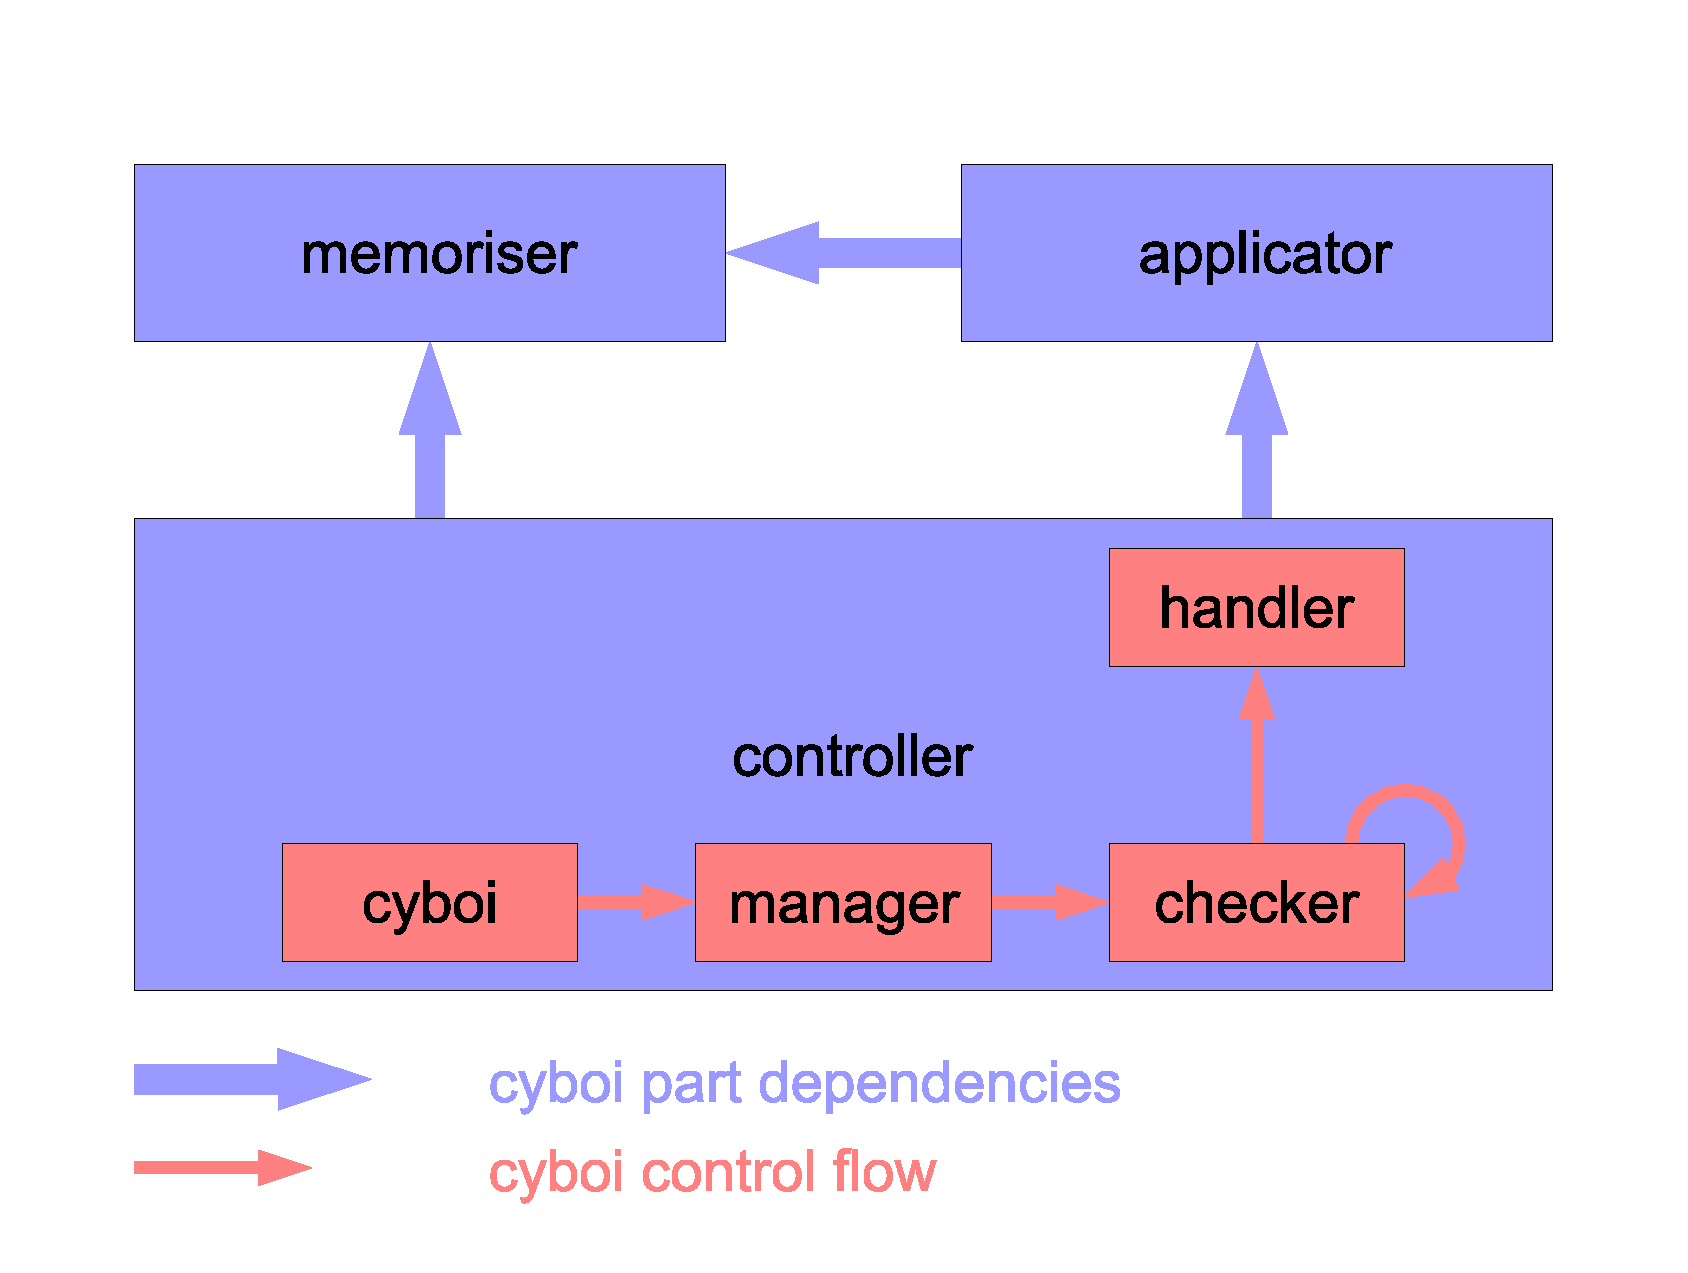
\includegraphics[scale=0.2]{vector/dependencies.eps}
        \caption{CYBOI Architecture}
        \label{cyboi_figure}
    \end{center}
\end{figure}

Figure \ref{cyboi_figure} shows three main parts of CYBOI: The
\emph{Controller} manages system startup, shutdown and the handling of signals
during its runtime; the system uses just one central signal checking loop. The
\emph{Memoriser} provides memory structures (to store knowledge) and procedures
to access these. Logic knowledge is processed in the \emph{Applicator}.
Parallels to the \emph{von Neumann} architecture \cite{selflinux} are intended.
